
\documentclass[letterpaper,hide notes,xcolor={table,svgnames},pdftex,10pt]{beamer}
\def\showexamples{t}

\usecolortheme{crane}
\setbeamertemplate{navigation symbols}{}

\usetheme{MyPittsburgh}
\usepackage{hyperref}
\usepackage{graphicx,xspace}
\usepackage[normalem]{ulem}
\usepackage{multicol}
\usepackage{amsmath,amssymb,amsthm,graphicx,xspace}
\newcommand\SF[1]{$\bigstar$\footnote{SF: #1}}

\usepackage[sfdefault,lf]{carlito}
\usepackage[T1]{fontenc}
\usepackage[scaled]{beramono}
\usepackage{tikzpagenodes}
\newcommand{\Rplus}{\protect\hspace{-.1em}\protect\raisebox{.35ex}{\small{\small\textbf{+}}}}
\newcommand{\Cpp}{\mbox{C\Rplus\Rplus}\xspace}

\newcounter{tmpnumSlide}
\newcounter{tmpnumNote}

\newcommand\mnote[1]{%
	\addtocounter{tmpnumSlide}{1}
	\ifdefined\showcues {~\tiny\fbox{\arabic{tmpnumSlide}}}\fi
	\note{\setlength{\parskip}{1ex}\addtocounter{tmpnumNote}{1}\textbf{\Large \arabic{tmpnumNote}:} {#1\par}}}

\newcommand\mmnote[1]{\note{\setlength{\parskip}{1ex}#1\par}}


\newcommand\mquestion[2]{{~\color{red}\fbox{?}}\note{\setlength{\parskip}{1ex}\par{\Large \textbf{?}} #1} \note{\setlength{\parskip}{1ex}\par{\Large \textbf{A}} #2\par}\ifdefined \presentationonly \pause \fi}

\newcommand\blackboard[1]{%
	\ifdefined   \showblackboard
		{#1}
	\else {\begin{center} \fbox{\colorbox{blue!30}{%
						\begin{minipage}{.95\linewidth}%
							\hspace{\stretch{1}} Some space intentionally left blank; done at the blackboard.%
						\end{minipage}}}\end{center}}%
	\fi%
}

\usepackage{listings}
\lstset{%
	keywordstyle=\bfseries,
	aboveskip=15pt,
	belowskip=15pt,
	captionpos=b,
	identifierstyle=\ttfamily,
	frame=lines,
	numbers=left, basicstyle=\scriptsize, numberstyle=\tiny, stepnumber=0, numbersep=2pt}

\usepackage{siunitx}
\newcommand\sius[1]{\num[group-separator = {,}]{#1}\si{\micro\second}}
\newcommand\sims[1]{\num[group-separator = {,}]{#1}\si{\milli\second}}
\newcommand\sins[1]{\num[group-separator = {,}]{#1}\si{\nano\second}}
\sisetup{group-separator = {,}, group-digits = true}

%% -------------------- tikz --------------------
\usepackage{tikz}
\usetikzlibrary{positioning}
\usetikzlibrary{arrows,backgrounds,automata,decorations.shapes,decorations.pathmorphing,decorations.markings,decorations.text}

\tikzstyle{place}=[circle,draw=blue!50,fill=blue!20,thick, inner sep=0pt,minimum size=6mm]
\tikzstyle{transition}=[rectangle,draw=black!50,fill=black!20,thick, inner sep=0pt,minimum size=4mm]

\tikzstyle{block}=[rectangle,draw=black, thick, inner sep=5pt]
\tikzstyle{bullet}=[circle,draw=black, fill=black, thin, inner sep=2pt]

\tikzstyle{pre}=[<-,shorten <=1pt,>=stealth',semithick]
\tikzstyle{post}=[->,shorten >=1pt,>=stealth',semithick]
\tikzstyle{bi}=[<->,shorten >=1pt,shorten <=1pt, >=stealth',semithick]

\tikzstyle{mut}=[-,>=stealth',semithick]

\tikzstyle{treereset}=[dashed,->, shorten >=1pt,>=stealth',thin]

\usepackage{ifmtarg}
\usepackage{xifthen}
\makeatletter
% new counter to now which frame it is within the sequence
\newcounter{multiframecounter}
% initialize buffer for previously used frame title
\gdef\lastframetitle{\textit{undefined}}
% new environment for a multi-frame
\newenvironment{multiframe}[1][]{%
	\ifthenelse{\isempty{#1}}{%
		% if no frame title was set via optional parameter,
		% only increase sequence counter by 1
		\addtocounter{multiframecounter}{1}%
	}{%
		% new frame title has been provided, thus
		% reset sequence counter to 1 and buffer frame title for later use
		\setcounter{multiframecounter}{1}%
		\gdef\lastframetitle{#1}%
	}%
	% start conventional frame environment and
	% automatically set frame title followed by sequence counter
	\begin{frame}%
		\frametitle{\lastframetitle~{\normalfont(\arabic{multiframecounter})}}%
		}{%
	\end{frame}%
}
\makeatother

\makeatletter
\newdimen\tu@tmpa%
\newdimen\ydiffl%
\newdimen\xdiffl%
\newcommand\ydiff[2]{%
	\coordinate (tmpnamea) at (#1);%
	\coordinate (tmpnameb) at (#2);%
	\pgfextracty{\tu@tmpa}{\pgfpointanchor{tmpnamea}{center}}%
	\pgfextracty{\ydiffl}{\pgfpointanchor{tmpnameb}{center}}%
	\advance\ydiffl by -\tu@tmpa%
}
\newcommand\xdiff[2]{%
	\coordinate (tmpnamea) at (#1);%
	\coordinate (tmpnameb) at (#2);%
	\pgfextractx{\tu@tmpa}{\pgfpointanchor{tmpnamea}{center}}%
	\pgfextractx{\xdiffl}{\pgfpointanchor{tmpnameb}{center}}%
	\advance\xdiffl by -\tu@tmpa%
}
\makeatother
\newcommand{\copyrightbox}[3][r]{%
	\begin{tikzpicture}%
		\node[inner sep=0pt,minimum size=2em](ciimage){#2};
		\usefont{OT1}{phv}{n}{n}\fontsize{4}{4}\selectfont
		\ydiff{ciimage.south}{ciimage.north}
		\xdiff{ciimage.west}{ciimage.east}
		\ifthenelse{\equal{#1}{r}}{%
			\node[inner sep=0pt,right=1ex of ciimage.south east,anchor=north west,rotate=90]%
			{\raggedleft\color{black!50}\parbox{\the\ydiffl}{\raggedright{}#3}};%
		}{%
			\ifthenelse{\equal{#1}{l}}{%
				\node[inner sep=0pt,right=1ex of ciimage.south west,anchor=south west,rotate=90]%
				{\raggedleft\color{black!50}\parbox{\the\ydiffl}{\raggedright{}#3}};%
			}{%
				\node[inner sep=0pt,below=1ex of ciimage.south west,anchor=north west]%
				{\raggedleft\color{black!50}\parbox{\the\xdiffl}{\raggedright{}#3}};%
			}
		}
	\end{tikzpicture}
}


%% --------------------

%\usepackage[excludeor]{everyhook}
%\PushPreHook{par}{\setbox0=\lastbox\llap{MUH}}\box0}

%\vspace*{\stretch{1}

%\setbox0=\lastbox \llap{\textbullet\enskip}\box0}

\setlength{\parskip}{\fill}

\newcommand\noskips{\setlength{\parskip}{1ex}}
\newcommand\doskips{\setlength{\parskip}{\fill}}

\newcommand\xx{\par\vspace*{\stretch{1}}\par}
\newcommand\xxs{\par\vspace*{2ex}\par}
\newcommand\tuple[1]{\langle #1 \rangle}
\newcommand\code[1]{{\sf \footnotesize #1}}
\newcommand\ex[1]{\uline{Example:} \ifdefined \presentationonly \pause \fi
	\ifdefined\showexamples#1\xspace\else{\uline{\hspace*{2cm}}}\fi}

\newcommand\ceil[1]{\lceil #1 \rceil}


\AtBeginSection[]
{
	\begin{frame}
		\frametitle{Outline}
		\tableofcontents[currentsection]
	\end{frame}
}



\pgfdeclarelayer{edgelayer}
\pgfdeclarelayer{nodelayer}
\pgfsetlayers{edgelayer,nodelayer,main}

\tikzstyle{none}=[inner sep=0pt]
\tikzstyle{rn}=[circle,fill=Red,draw=Black,line width=0.8 pt]
\tikzstyle{gn}=[circle,fill=Lime,draw=Black,line width=0.8 pt]
\tikzstyle{yn}=[circle,fill=Yellow,draw=Black,line width=0.8 pt]
\tikzstyle{empty}=[circle,fill=White,draw=Black]
\tikzstyle{bw} = [rectangle, draw, fill=blue!20,
text width=4em, text centered, rounded corners, minimum height=2em]

\newcommand{\CcNote}[1]{% longname
	This work is licensed under the \textit{Creative Commons #1 3.0 License}.%
}
\newcommand{\CcImageBy}[1]{%
	\includegraphics[scale=#1]{creative_commons/cc_by_30.pdf}%
}
\newcommand{\CcImageSa}[1]{%
	\includegraphics[scale=#1]{creative_commons/cc_sa_30.pdf}%
}
\newcommand{\CcImageNc}[1]{%
	\includegraphics[scale=#1]{creative_commons/cc_nc_30.pdf}%
}
\newcommand{\CcGroupBySa}[2]{% zoom, gap
	\CcImageBy{#1}\hspace*{#2}\CcImageNc{#1}\hspace*{#2}\CcImageSa{#1}%
}
\newcommand{\CcLongnameByNcSa}{Attribution-NonCommercial-ShareAlike}

\newenvironment{changemargin}[1]{% 
	\begin{list}{}{% 
		\setlength{\topsep}{0pt}% 
		\setlength{\leftmargin}{#1}% 
		\setlength{\rightmargin}{1em}
		\setlength{\listparindent}{\parindent}% 
		\setlength{\itemindent}{\parindent}% 
		      \setlength{\parsep}{\parskip}% 
		      }% 
		\item[]}{\end{list}}




\title{Lecture 5 --- Process State}

\author{Jeff Zarnett \\ \small \texttt{jzarnett@uwaterloo.ca}}
\institute{Department of Electrical and Computer Engineering \\
  University of Waterloo}
\date{\today}


\begin{document}

\begin{frame}
  \titlepage

 \end{frame}

\begin{frame}
\frametitle{Process State}

The OS is responsible for determining which programs run when.\\
\quad ...and how to allocate resources.

The current state of the process is therefore important.

To maintain the state, there is a variable in the PCB.

We will think of this as a finite state machine (FSM).

\end{frame}

\begin{frame}
\frametitle{Two State Model}
Let us begin with the simplest possible model: 2 states.

\begin{enumerate}
	\item \textbf{Running}
	\item \textbf{Not Running}
\end{enumerate}


\end{frame}

\begin{frame}
\frametitle{Two State Model}

\begin{center}
\includegraphics[width=0.9\textwidth]{images/2-state-model.png}
\end{center}

\end{frame}

\begin{frame}
\frametitle{Two State Model}

There are the following transitions in the diagram:
\begin{itemize}
	\item \textbf{Create}
	\item \textbf{Dispatch}
	\item \textbf{Suspend}
	\item \textbf{Exit}
\end{itemize}

\end{frame}

\begin{frame}
\frametitle{Two State Model}
This simple model is inadequate.

It assumes every process is constantly ready to run.

We need a way to indicate a process is not ready to run...

\end{frame}

\begin{frame}
\frametitle{Three State Model}

A program that requests a resource may not get it right away. 

This is not to say the program will never get it.\\
\quad It's just that it does not have it right now. 

The program wants to continue but can't until it gets what it's waiting for. 

If the scheduler picks a process that is waiting for user input:\\
\quad Nothing will be happening while the program is waiting for input.\\
\quad The CPU's time would be wasted. 

Third state: ``not ready to proceed''.


\end{frame}

\begin{frame}
\frametitle{Three State Model}

\begin{enumerate}
 \item \textbf{Running}
 \item \textbf{Ready}
 \item \textbf{Blocked}
\end{enumerate}

The scheduler will not choose a blocked process.

\end{frame}

\begin{frame}
\frametitle{Three State Model}

Processes get blocked when they are \textit{waiting} for something.

Suppose process $P_{n}$ is waiting for user input. 

When the user input is received, an interrupt is generated.

The handler takes the input from the I/O device (keyboard), delivers it to $P_{n}$, then moves the state of $P_{n}$ to ``Ready''.

\end{frame}

\begin{frame}
\frametitle{Three State Model}

\begin{center}
\includegraphics[width=0.9\textwidth]{images/3-state-model.png}
\end{center}


\end{frame}

\begin{frame}
\frametitle{Three State Model}

There are six transitions in the diagram:
\begin{itemize}
	\item \textbf{Create}
	\item \textbf{Dispatch}
	\item \textbf{Suspend}
	\item \textbf{Exit}
	\item \textbf{Block}
	\item \textbf{Unblock}
\end{itemize}

\end{frame}

\begin{frame}
\frametitle{Five State Model}

The three state model is good, but it does not cover things like zombies.\\
\quad Life pro tip: the character who doubts that zombies are real dies first.

A UNIX process may be finished but its value yet uncollected.

It is not ready to run, but not waiting for a resource either.

New state to add, then: ``Terminated\footnote{Say this in Arnold Schwarzenegger's voice}'' -- finished but not cleaned up.

\end{frame}

\begin{frame}
\frametitle{Five State Model}
That accounts for four states; what about the fifth?

The fifth is the ``New'' state: just created.

If the user creates a process, the OS has significant work to do.\\
\quad Define an identifier.\\
\quad Instantiate the PCB.\\
\quad Put the process in the New state.

The process is defined, but the OS has not started it yet.

\end{frame}

\begin{frame}
\frametitle{Five State Model}
Why bother with the ``New'' state?

The system may limit the number of concurrent processes.

New processes are typically on disk and not in memory.

\end{frame}

\begin{frame}
\frametitle{Five State Model}

Thus, with the two new states added, the five states are:

\begin{enumerate}
 \item \textbf{Running}
 \item \textbf{Ready}
 \item \textbf{Blocked}
 \item \textbf{New}
 \item \textbf{Terminated}
\end{enumerate}

\end{frame}

\begin{frame}
\frametitle{Five State Model}

\begin{center}
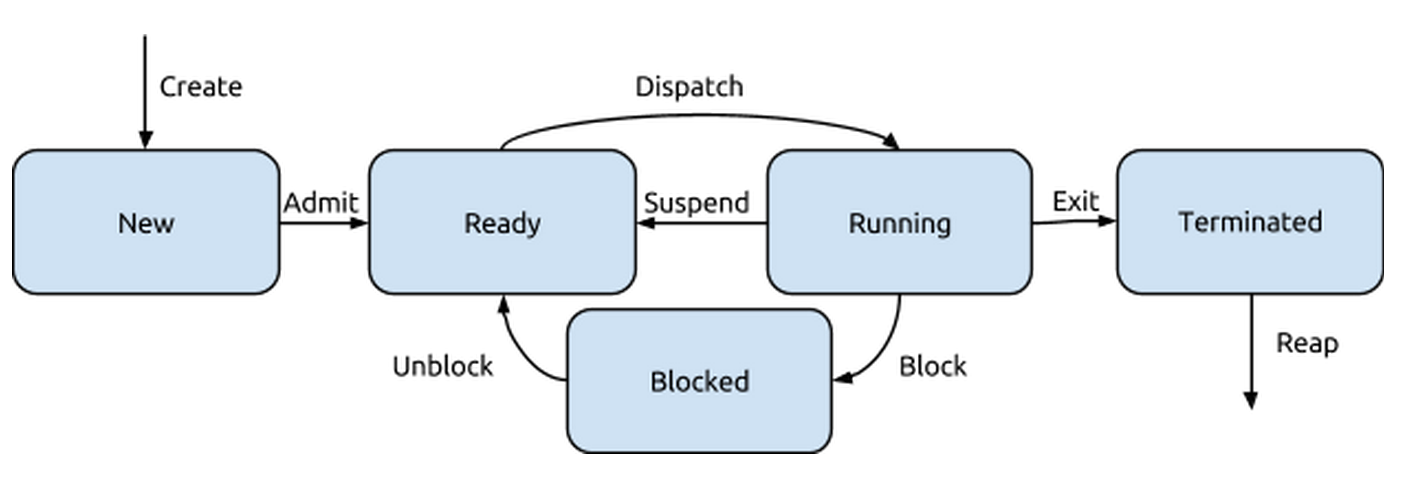
\includegraphics[width=0.9\textwidth]{images/5-state-model.png}
\end{center}

\end{frame}

\begin{frame}
\frametitle{Five State Model}

There are now eight transitions:

\begin{itemize}
	\item \textbf{Create}
	\item \textbf{Admit}
	\item \textbf{Dispatch}
	\item \textbf{Suspend}
	\item \textbf{Exit}
	\item \textbf{Block}
	\item \textbf{Unblock}
	\item \textbf{Reap}
\end{itemize}

\end{frame}

\begin{frame}
\frametitle{Five State Model}

There are two additional exit transitions that are not shown.

A process can go directly from ``Ready'' or ``Blocked'' to ``Terminated''.

This happens if a process is killed.


\end{frame}

\begin{frame}
\frametitle{More is the New More}

We can expand on the five state model by considering disk.

A process maybe swapped out to disk rather than in main memory.

If an executing process gets blocked, maybe swap it to disk.

Users often want more processes running than fit in memory.

The problem is not the PCBs, but stack \& heap space of the programs.

\end{frame}

\begin{frame}
\frametitle{Don't Even Start...}

A (non-)solution: do not start a program when insufficient memory.

Programs do not declare how much memory they will use.

They may not even know themselves -- how could Microsoft Word know what document the user plans to open and edit?

Imagine being told a program cannot launch due to low memory.\\
\quad User complaints about ``random'' refusal to launch.

\end{frame}

\begin{frame}
\frametitle{Let's Throw Money at the Problem!}

Another (non-)solution, then: buy more RAM. 

Memory gets too expensive beyond a certain point.

But: ``programs expand to fill the RAM available''.

Computers might have 1000$\times$ more RAM than it did 20 years ago, but programs today use 1000$\times$ more RAM than the programs of 20 years ago. 

Increase the size of memory leads to larger, not more, processes.

\end{frame}

\begin{frame}
\frametitle{The Last Resort: Disk}

With no other place to put them, we have to put some processes on disk.

This is what we know as \alert{swapping}.

When the demands for memory exceed the available memory, some of the processes will be moved to disk storage to make room. 

This is a notably expensive operation.
\end{frame}

\begin{frame}
\frametitle{Swapping to Disk}

Swapping a process to disk might mean transferring several hundred megabytes of data, or even a few gigabytes. 

This, from the perspective of the CPU, takes about seven eternities. 

Then, when that process is going to run again, we need to load it back in to memory, which will take just as much time as it took to flush it out. 

So this is something to be done only when necessary.

\end{frame}

\begin{frame}
\frametitle{The Sixth Sens...State}

We do not want to spend any more time swapping the process in and out of memory than is necessary.

 We need to know if a particular process is in memory or on disk.
 
Thus we need a new state: swapped.  

Ideally, we will only swap a process to disk if it is blocked. 

A process swapped to disk then enters that sixth state, swapped.\\
\quad It is blocked and not in main memory.

\end{frame}

\begin{frame}
\frametitle{Lucky Number Seven}

There are two scenarios that tell us that six is not sufficient.

1. What if all processes are ready, but there is a memory space shortage?

2. What if the event a swapped process waited for took place?

Avoid bringing in a swapped process if it is just going to be blocked.

Solution: split swapped into ``Ready/Swapped''and ``Blocked/Swapped''.

\end{frame}

\begin{frame}
\frametitle{Seven State Model}

\begin{center}
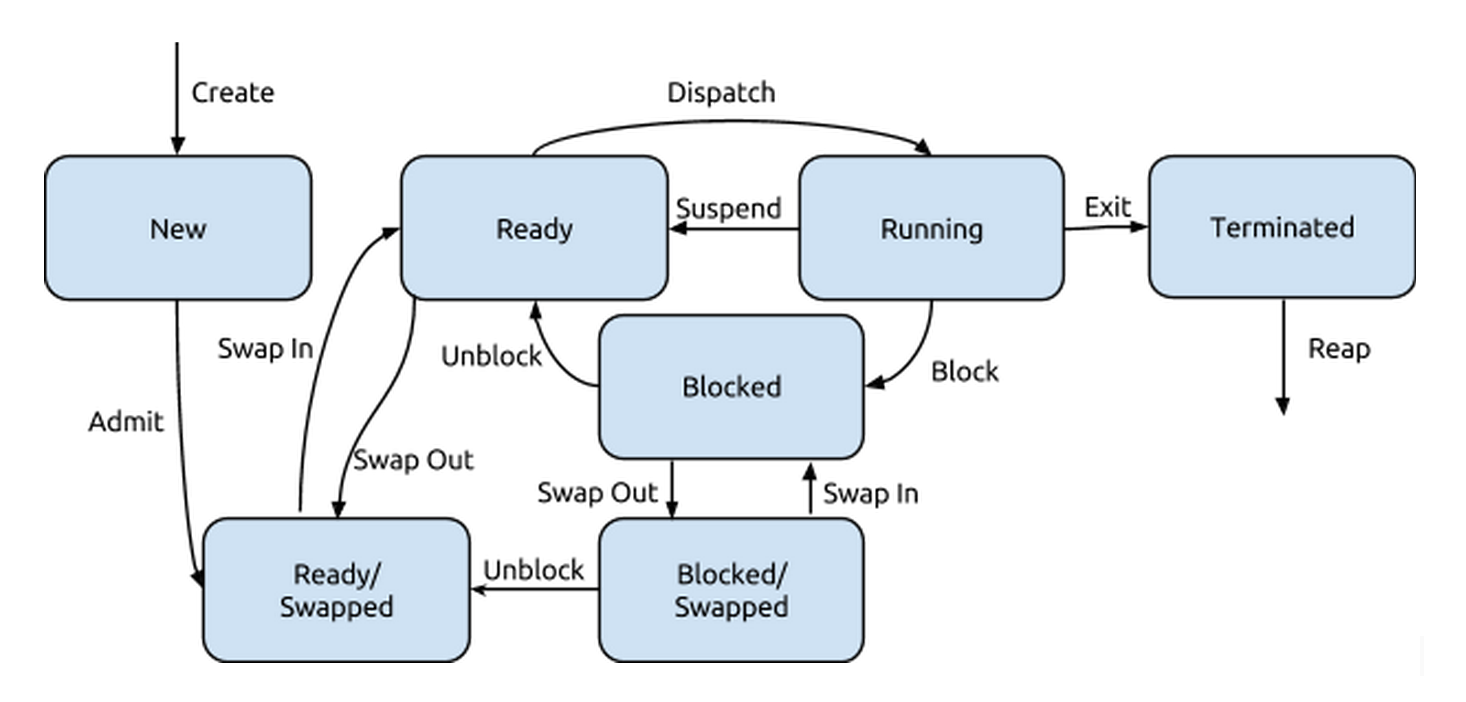
\includegraphics[width=0.9\textwidth]{images/7-state-model.png}
\end{center}

\end{frame}

\begin{frame}
\frametitle{Seven State Model}
A variant of the five state model.

The ``Admit'' transition is modified: by default the new process does not start in main memory.

Two new transitions: ``Swap In'' and ``Swap Out''.

A second ``Unblock'' transition.

As in the five state model, some additional ``Exit'' transitions.

\end{frame}




\begin{frame}
\frametitle{A Preview of Scheduling}

Processes, represented by their PCB, are maintained in a data structure; typically a linked list or a queue of some sort. 

For efficiency reasons, it would not make sense to have all processes in one single linked list that we would have to iterate over. 

If there are 200 processes and the next ready one is number 137...

So it is logical to take non-ready processes out of this list.

\end{frame}



\begin{frame}
\frametitle{E Pluribus... Pluribum?}

When a process is in some state like ``Blocked'', where does it go? 

This is a question we will come back to when we discuss scheduling.

But for now, it's convenient for the operating system to keep track of what processes are in which states separately. 

If a process is waiting for a disk operation, when the disk becomes available, it would be convenient to know quickly what processes are waiting for the disk.

\end{frame}



\begin{frame}
\frametitle{PCBs in Queues}

\begin{center}
\includegraphics[width=0.65\textwidth]{images/pcbs-in-queues.png}
\end{center}

\end{frame}



\begin{frame}
\frametitle{Queueing Diagram}

\begin{center}
\includegraphics[width=0.75\textwidth]{images/queueing-diagram.png}
\end{center}


\end{frame}

\end{document}

